Figure \ref{fig: l2 errors test 1} shows the $L^2$ error of all performances of the first test case that have converged, the polynomial degrees $k$ were taken to be $1,\dots,3$ and $k_{DH}$ equal to all variants $0, \dots, k$. In Figure \ref{fig: h1 errors test 1} the corresponding $H^1$ errors are plotted.
\begin{figure}[H]
\centering
	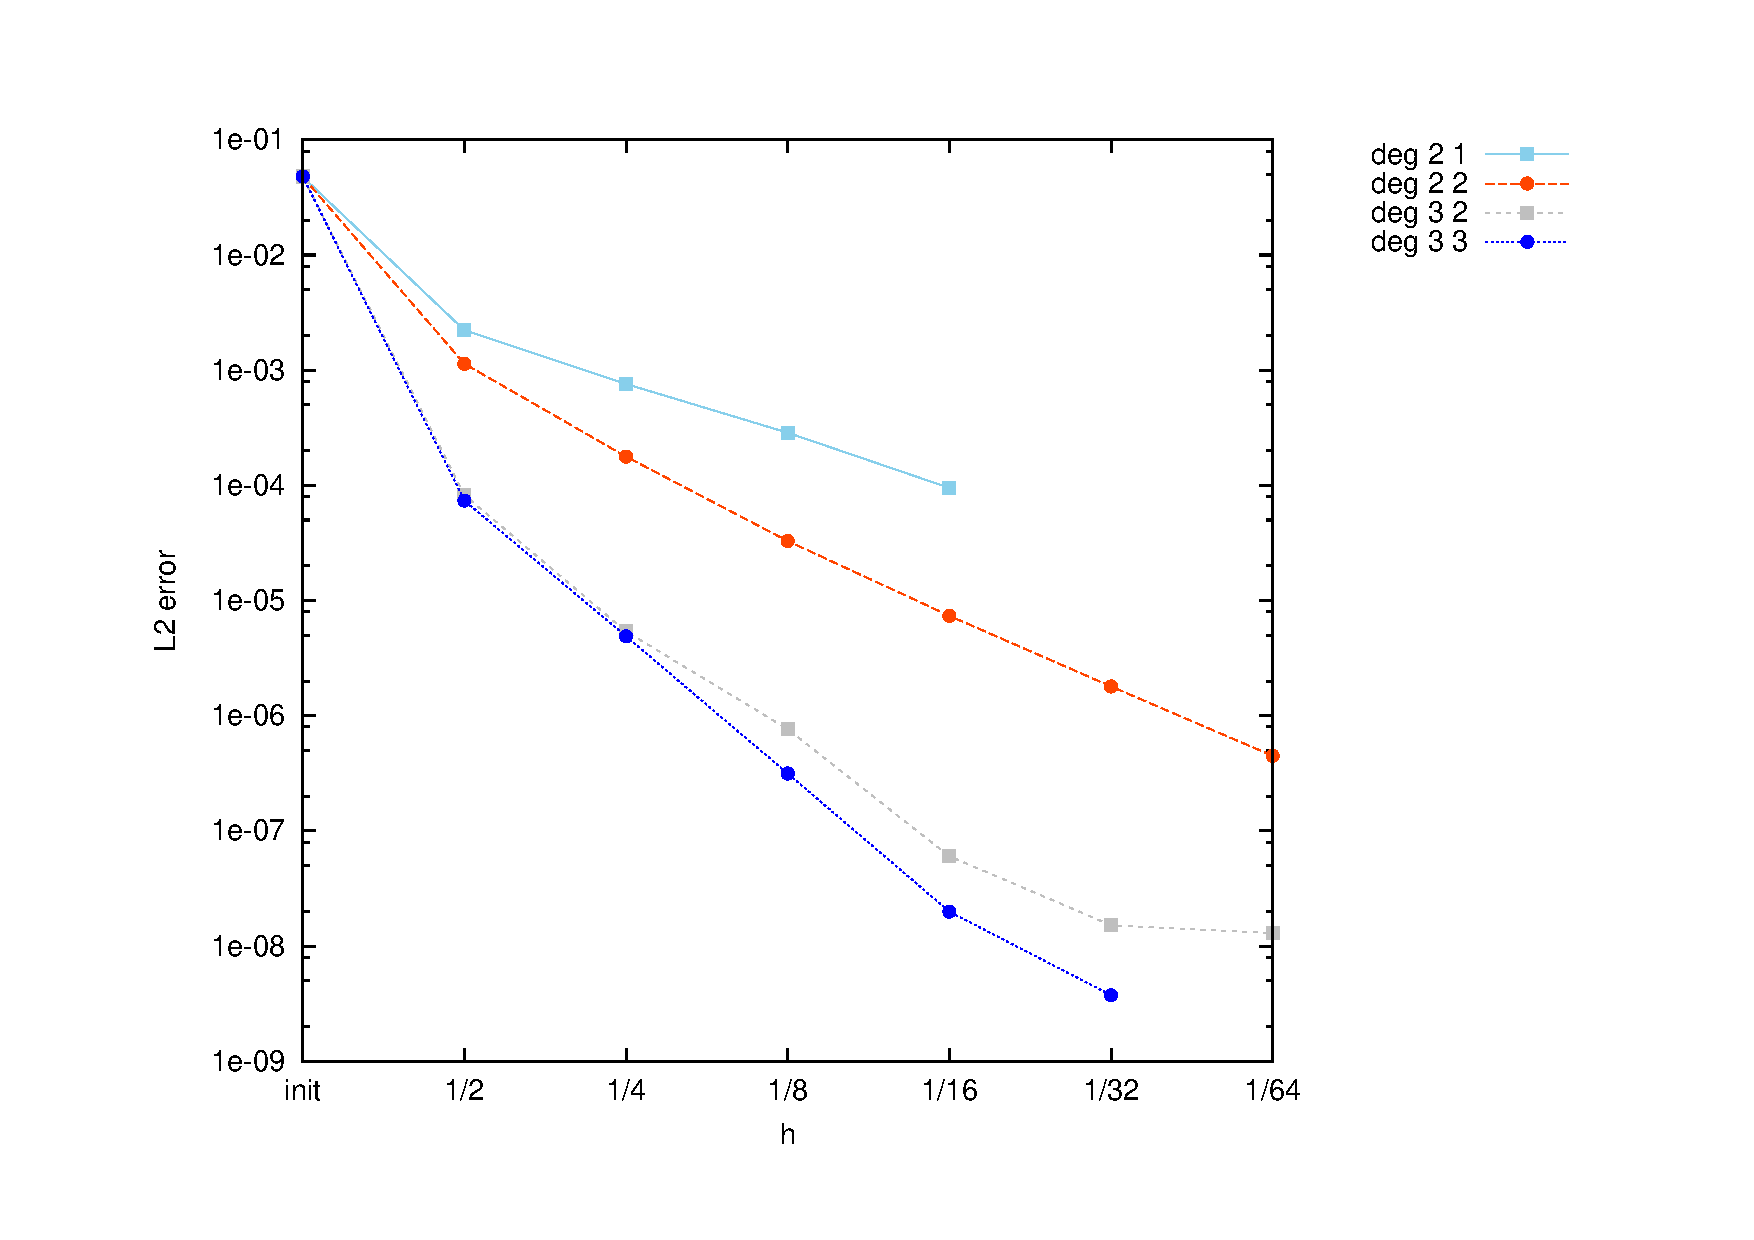
\includegraphics[scale =0.4]{../../FEniCS/diagrams/MA1_Neilan_l2.pdf}
	\caption{$L^2$ errors for test case \ref{test smooth}}
	\label{fig: l2 errors test 1}
\end{figure}
\begin{figure}[H]
\centering
	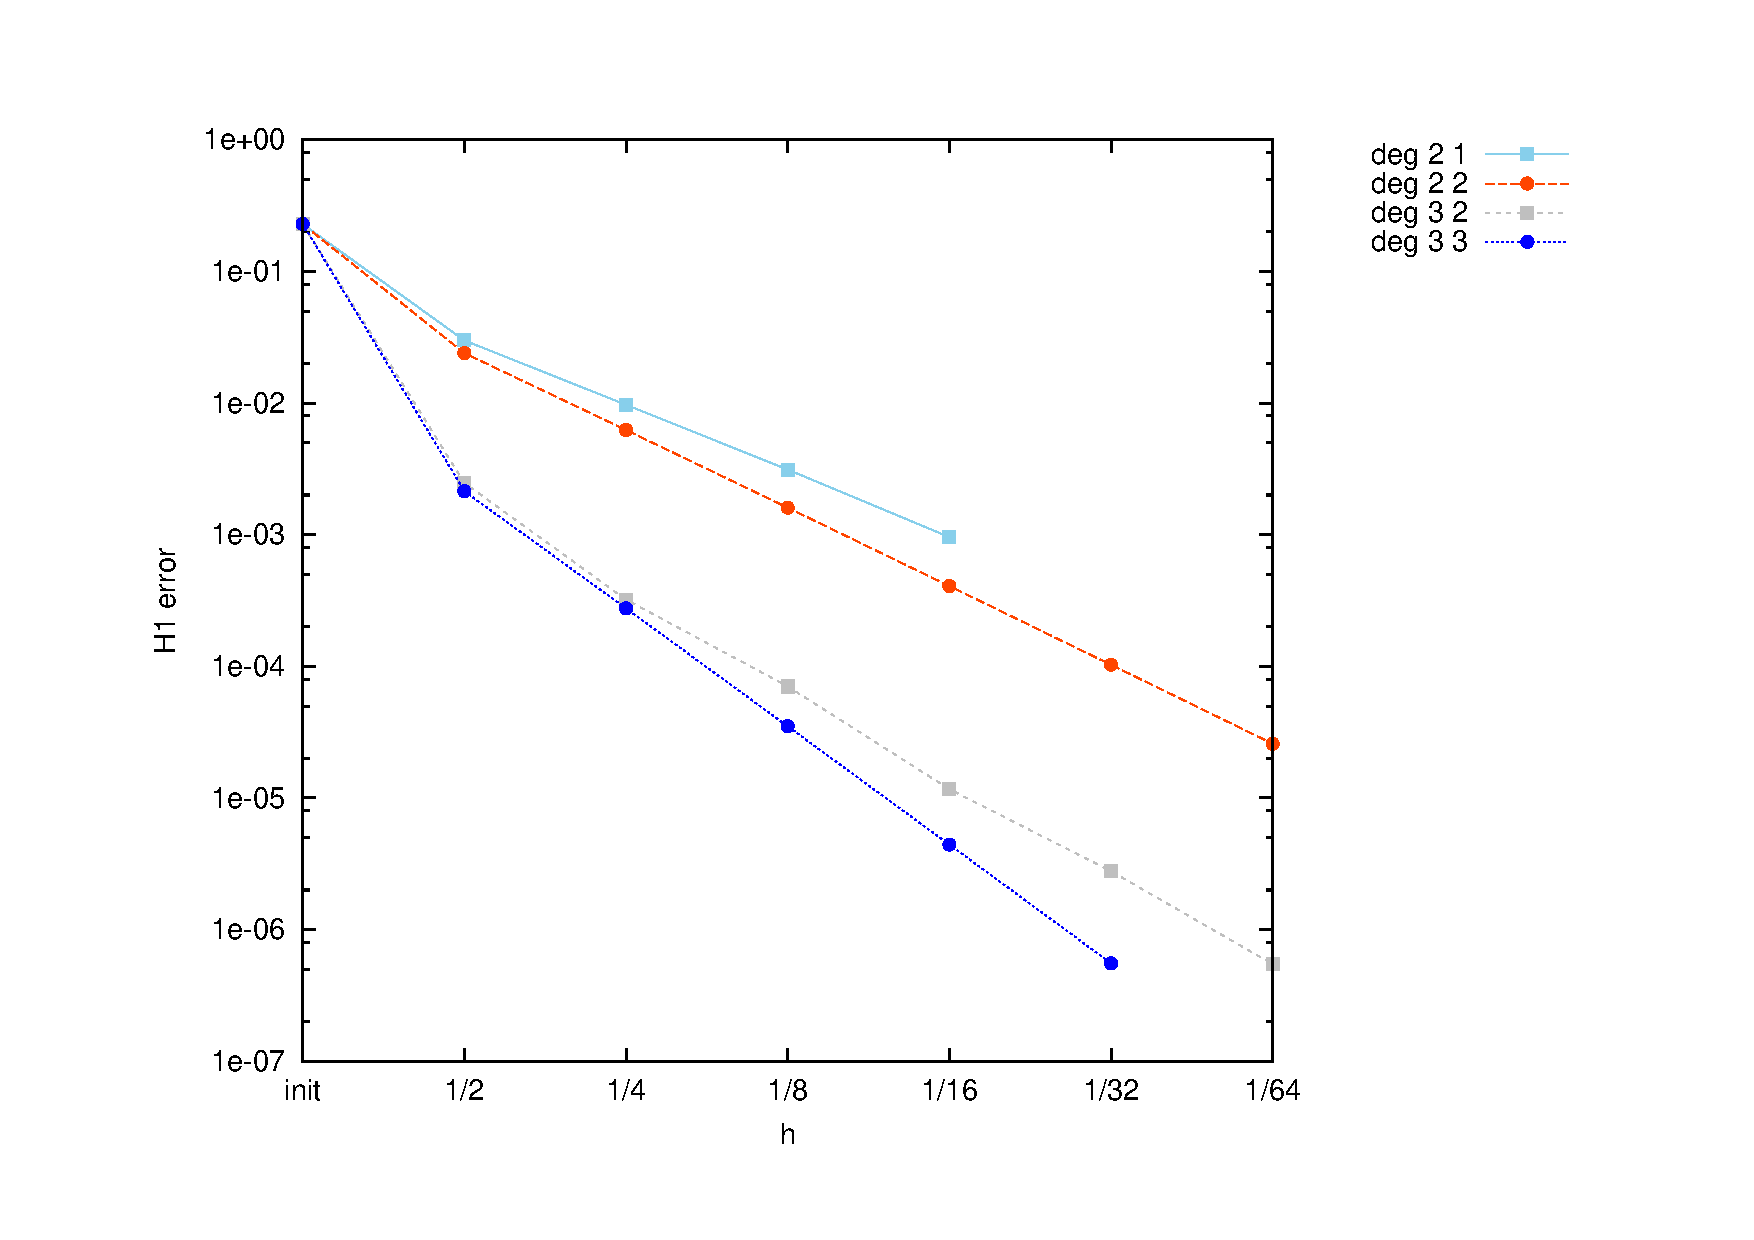
\includegraphics[scale =0.4]{../../FEniCS/diagrams/MA1_Neilan_h1.pdf}
	\caption{$H^1$ errors for test case \ref{test smooth}}
	\label{fig: h1 errors test 1}
\end{figure}

Due to the large number of degree of freedoms the I could not obtain any results for the cases $k=2,3$ and $k_{DH}=2,3$ on the finest grid, for $k=3$ and $k_{DH}=3$ even on a mesh with $h=1/64$ the requested memory was too much.

As also experienced by Neilan the method does not work for the polynomial degree $k=1$. Similarly, in runs with a low polynomial degree $k_{DH}$ Newton's method did not converge. \todo{LU hat nicht funktioniert}
The results for the runs with $k=3$ are shown more detailed in Table \ref{tab: l2 errors test 1 deg 2}, in both tables the column $N$ refers to the number of iterations the Newton solver needed to reach the desired tolerance. 
\begin{table}[H]
	\begin{subtable}[b]{0.45\textwidth}
		\centering
		\pgfplotstabletypeset[columns={iterations, l2error, h1error,N},
				    every row 0 column 0/.style={set content=init},
		]\MAOnedegThreeThree
    	\caption{Error for $k=3, k_{DH}=3$}
   \end{subtable}
   ~
	\begin{subtable}[b]{0.45\textwidth}
		\centering
		\pgfplotstabletypeset[columns={iterations, l2error, h1error,N},
				    every row 0 column 0/.style={set content=init},
		]\MAOnedegThreeTwo
 	\caption{Error for $k=3, k_{DH}=2$}
	\end{subtable}
	\caption{Errors for test case \ref{test smooth}}
	\label{tab: l2 errors test 1 deg 2}
\end{table}
Considering this results in the smooth test scenario we observe that the error almost do not alter for different polynomial degrees $k_{DH}$ if both converge. Albeit for fine grids the methods with less difference between the two degrees seem to perform better. The calculated numerical orders as shown in table \ref{tab: order} supports this first intuition.

\begin{table}[H]
\begin{subtable}[b]{0.45\textwidth}
\centering
	\pgfplotstabletypeset
	{
		k $k_{DH}$ {numerical order}
		2 1  1.50338
		2 2  2.24427
		3 2 2.63597
		3 3 3.64758
	}
	\caption{numerical order in $L2$ norm}
\end{subtable}
\begin{subtable}[b]{0.45\textwidth}
	\pgfplotstabletypeset
	{
		k $k_{DH}$ {numerical order}
		2 1  1.65382 
		2 2  1.973
		3 2 2.39616
		3 3 2.97876
	}
	\caption{numerical order in $H1$ norm}
	\end{subtable}
\caption{numerical order in test \ref{test smooth}}
\label{tab: order}
\end{table}

This test scenario was also performed with the additional normal jump penalty term as stated in \eqref{eq: neilan eq1 + jump} weighted with $\eta$ equal to 50 leading to the results shown in figure \ref{fig: l2 errors test 1 jump} and the tables \ref{tab: l2 errors test 1 deg 2 jump}.

\begin{figure}[h!]
\centering
	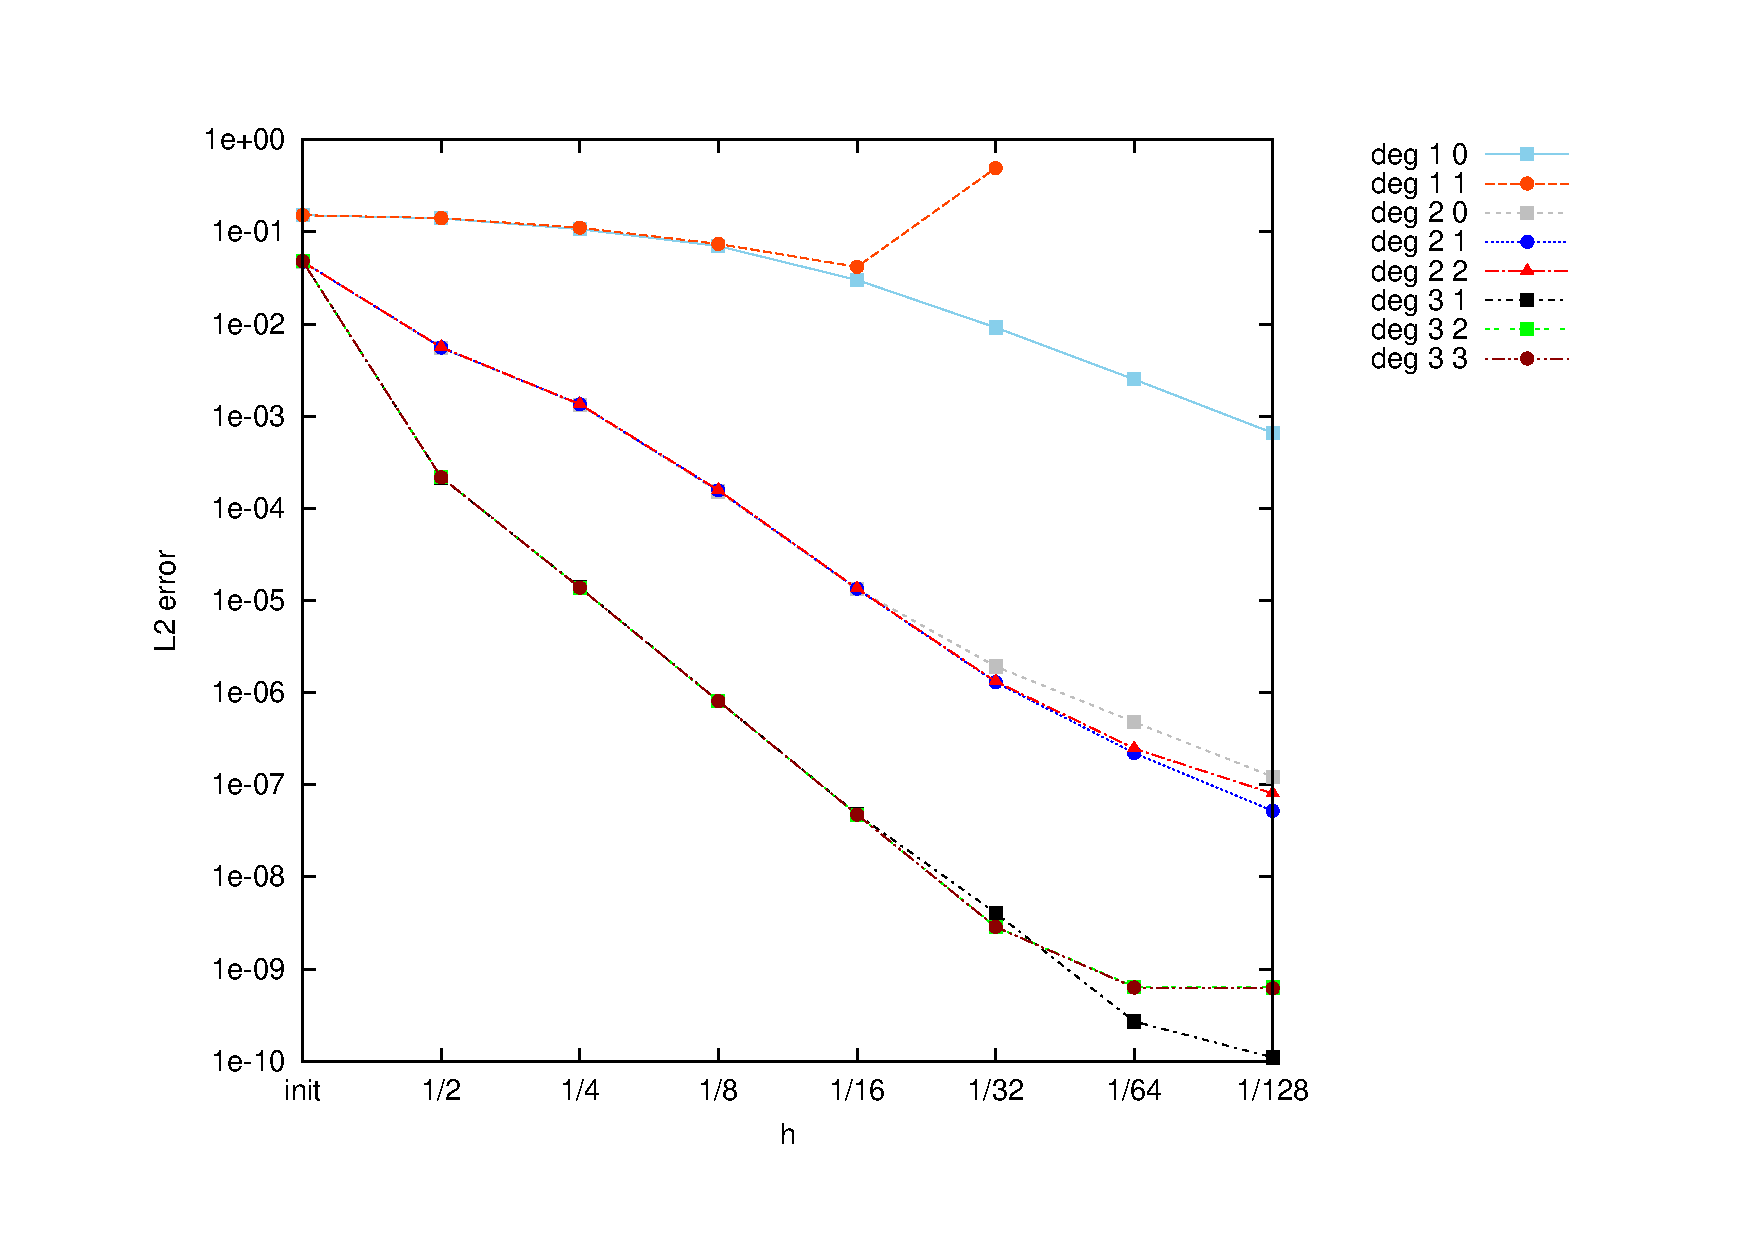
\includegraphics[scale=0.4]{../../FEniCS/diagrams/MA1_Neilan_GradJump_l2.pdf}
	\caption{$L^2$ errors for test case \ref{test smooth} and additional gradient jump penalty}
	\label{fig: l2 errors test 1 jump}
\end{figure}

\begin{figure}[H]
\centering
	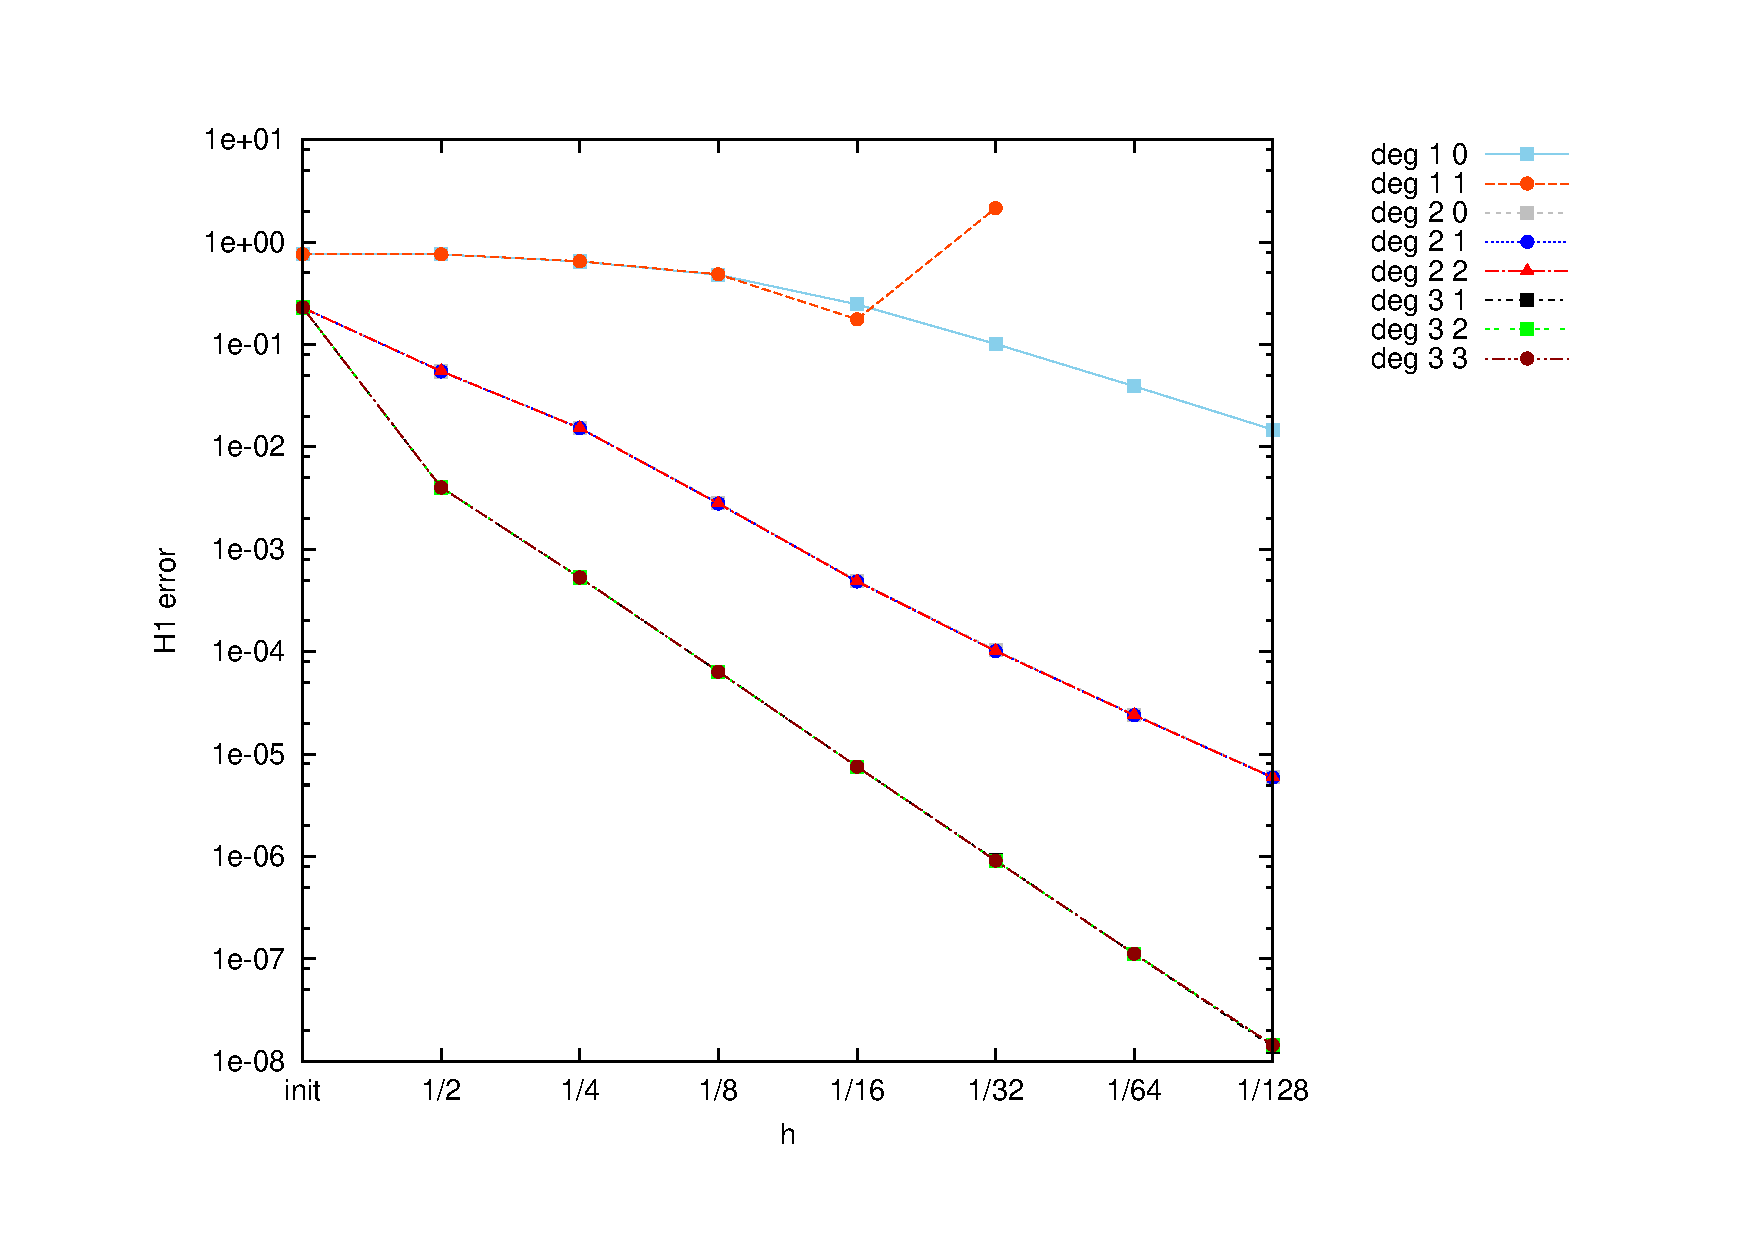
\includegraphics[scale =0.4]{../../FEniCS/diagrams/MA1_Neilan_GradJump_h1.pdf}
	\caption{$H^1$ errors for test case \ref{test smooth} and additional gradient jump penalty}
	\label{fig: h1 errors test 1 jump}
\end{figure}
\begin{table}[H]
	\begin{subtable}[b]{0.45\textwidth}
		\centering
		\pgfplotstabletypeset[
		columns={iterations, l2error, h1error,N},
		    every row 0 column 0/.style={set content=init},
		    every row 7 column 1/.style={set content={-}},
		    every row 7 column 2/.style={set content={-}},
		    every row 7 column 3/.style={set content={-}},
		]\MAOneJumpdegTwoTwo
    	\caption{Error for $k=2, k_{DH}=2$}
   \end{subtable}
   ~
	\begin{subtable}[b]{0.45\textwidth}
		\centering
		\pgfplotstabletypeset[columns={iterations, l2error, h1error,N},
		    every row 0 column 0/.style={set content=init},
		]\MAOneJumpdegTwoZero
	\caption{Error for $k=2, k_{DH}=0$}
	\end{subtable}
	\caption{Errors for test case \ref{test smooth}}
	\label{tab: l2 errors test 1 deg 2 jump}
\end{table}
As claimed by Neilan the additional penalisation leads to a convergend method even for low polynomial degrees, even in the cases where only $k_{DH}$ was taken to be small. The calculated error norms indicate more clearly than in the non penalised runs that variation of $k_{DH}$ yields only to a slight loss of accuracy. The corresponding numerical orders can be found in \ref{tab: order jump}.
\begin{table}[H]
\centering
\begin{subtable}[b]{0.45\textwidth}
	\pgfplotstabletypeset
	{
		k $k_{DH}$ {numerical order}
		1 0 1.32061
		2 0 2.69871
		2 1 2.93488
		2 2 3.0406
		3 1 3.63116
		3 2 4.01895
		3 3 4.0588
	}
	\caption{numerical order in $L2$ norm}
	\end{subtable}
	\begin{subtable}[b]{0.45\textwidth}
	\pgfplotstabletypeset
	{
		k $k_{DH}$ {numerical order}
		1 0 0.978853
		2 0 2.24561
		2 1 2.24836
		2 2 2.28606
		3 1 3.03434
		3 2 3.0359
		3 3  3.0343
	}
	\caption{numerical order in $H1$ norm}
	\end{subtable}
	\caption{numerical order with jump penalty in test \ref{test smooth}}
\label{tab: order jump}
\end{table}
